
%(BEGIN_QUESTION)
% Copyright 2014, Tony R. Kuphaldt, released under the Creative Commons Attribution License (v 1.0)
% This means you may do almost anything with this work of mine, so long as you give me proper credit

Calculate the voltage dropped across the inductor, the capacitor, and the 8-ohm speaker in this sound system at the following frequencies, given a constant source voltage of 15 volts:

$$\includegraphics[width=15.5cm]{i01075x01.eps}$$

\begin{itemize}
\item{} $f =$ 200 Hz 
\item{} $f =$ 550 Hz 
\item{} $f =$ 900 Hz 
\end{itemize}

Regard the speaker as nothing more than an 8-ohm resistor.

\vskip 20pt \vbox{\hrule \hbox{\strut \vrule{} {\bf Suggestions for Socratic discussion} \vrule} \hrule}

\begin{itemize}
\item{} As part of an audio system, would this LC network tend to emphasize the {\it bass}, {\it treble}, or {\it mid-range} tones?
\end{itemize}

\underbar{file i01075}
%(END_QUESTION)





%(BEGIN_ANSWER)

\begin{itemize}
\item{} $f =$ 200 Hz ; $V_L =$ 1.750 V ; $V_C =$ 11.79 V ; $V_{speaker} =$ 5.572 V  
\item{} $f =$ 550 Hz ; $V_L =$ 6.472 V ; $V_C =$ 5.766 V ; $V_{speaker} =$ 7.492 V 
\item{} $f =$ 900 Hz ; $V_L =$ 9.590 V ; $V_C =$ 3.763 V ; $V_{speaker} =$ 6.783 V
\end{itemize}

This circuit is known as a {\it midrange crossover} in stereo system design.

%(END_ANSWER)





%(BEGIN_NOTES)

This is an interesting circuit to analyze.  Note how, out of the three frequency points we performed calculations at, the speaker's voltage is greatest at the {\it middle} frequency.  Note also how the inductor and capacitor drop very disparate amounts of voltage at the high and low frequencies.  Discuss this circuit's behavior with your students, and ask them what practical function this circuit performs.

%INDEX% Electronics review: AC reactance and impedance

%(END_NOTES)


